\documentclass{article}%
\usepackage[T1]{fontenc}%
\usepackage[utf8]{inputenc}%
\usepackage{lmodern}%
\usepackage{textcomp}%
\usepackage{lastpage}%
\usepackage{authblk}%
\usepackage{graphicx}%
%
\title{Caveolin{-}1 is a novel regulator of K{-}RAS{-}dependent migration in colon carcinogenesis}%
\author{Christopher Hale}%
\affil{Department of Oral Biology and Pathology, School of Dental Medicine, Stony Brook University, Stony Brook, New York, United States of America}%
\date{01{-}01{-}2008}%
%
\begin{document}%
\normalsize%
\maketitle%
\section{Abstract}%
\label{sec:Abstract}%
It's a phenomenon that scientists now believe affects us more than cells in our bodies, but the exact causes of it have been unclear.\newline%
Researchers from the University of California, Riverside are developing a new way to look at the interleukin{-}19 interleukin gene, which could lead to new treatments and theories.\newline%
"When you look at a normal human body, if there are any low levels of this cytokine, that results in an immune system reaction," said UC Riverside biologist Jessica Crane.\newline%
Low levels of interleukin{-}19 trigger an immune response and hampers our body's ability to fight disease. They also contribute to a buildup of oesophageal tumors, which can cause damage to the esophagus, but because they don't affect tissue formation it's often unclear how the gene influences it.\newline%
Biochemist Emily Kurtz has spent years studying interleukin{-}19 with Crane and are now building a "biophysics net" around the interleukin{-}19.\newline%
"There is a lot of evidence for this as a pathway," said Kurtz. "This is a pathway that we know very little about."\newline%
Kurtz said she discovered the interleukin{-}19 by attaching tiny imperfections to the amino acid a protein called orrin. The holes resemble the normal cells of mice but with an easily fixable surface and a structure a few tens of nanometers in diameter.\newline%
"That provides a really clear line for where it happens that this interleukin gene becomes active and inflammatory in cells," Kurtz said.\newline%
Researchers said this pathway may have other biological links, including that many of the cells inside the body are microfilarial, which also functions as a receptor for IL{-}19.\newline%
Crane said this method allows them to look at the interleukin{-}19 at its molecular level without altering the protein.\newline%
"Anything that has low interleukin expression, you can look at and see if it is inflammatory or if it is normal," Crane said.\newline%
Kurtz and Crane found several proteins that could be important markers in corneal inflammation or pancreatic tumor swelling.\newline%
The researchers said their next step will be to develop an invasive test that takes these tiny proteins and inserts them into cells of any age.\newline%
"What we're hoping is to reverse these inflammatory effects or modulate the progression of these inflammatory and pancreatic tumor (symptoms) and its other inflammatory effects," Crane said.\newline%
Biochemist James Smith is also hoping for a miracle fix using the findings of Crane and Kurtz.\newline%
"If we can control interleukin{-}19 then we can basically stop these inflammatory processes," Smith said.\newline%
The study was published recently in Science.

%
\subsection{Image Analysis}%
\label{subsec:ImageAnalysis}%


\begin{figure}[h!]%
\centering%
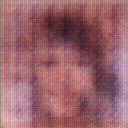
\includegraphics[width=150px]{500_fake_images/samples_5_240.png}%
\caption{A Close Up Of A Cat In A Room}%
\end{figure}

%
\end{document}